\documentclass[11pt,oneside]{article}
\usepackage[margin=1.0in]{geometry}
\usepackage[toc,page]{appendix}
\usepackage{graphicx}
\usepackage{setspace}
\usepackage{titlesec}
\usepackage[rgb]{xcolor}
\usepackage{verbatim}
\usepackage[square,sort,comma,numbers]{natbib}
\usepackage[hyphens,spaces,obeyspaces]{url}
\usepackage{tocbibind}
\usepackage{lipsum}
\usepackage{caption}
\usepackage{placeins}
\usepackage{enumerate}
\usepackage{enumitem}
\usepackage{amsgen, amsmath, amstext, amsbsy, amsthm, amsopn, tikz, amssymb}
\usepackage{fancyhdr}
\usepackage[colorlinks=true, urlcolor=blue,  linkcolor=blue, citecolor=blue]{hyperref}
\usepackage[colorinlistoftodos]{todonotes}
\usepackage{rotating}
\usepackage{subcaption}
\usepackage{tensor}
\usepackage[compat=1.1.0]{tikz-feynman}
\usepackage{mathtools}
\usepackage{tcolorbox}
\usepackage{physics}
\usepackage{bbm, bm}
\usepackage[utf8]{inputenc}
\hypersetup{linkcolor=blue, linktoc=page}
\newcommand{\approxtext}[1]{\ensuremath{\stackrel{\text{#1}}{\approx}}}
\newcommand{\musteq}{\ensuremath{\overset{!}{=}}}
\newcommand{\totd}{\ensuremath{\mathrm{d}}}

\title{\textbf{Continuous Variable Quantum Neural Networks} \\ \vspace{2mm} \large Brief Notes and Stuff}
\author{\textbf{Sangeet. S}}
\date{\today}

\newtheorem{theorem}{Theorem}[section]
\newtheorem{corollary}{Corollary}[theorem]
\newtheorem{lemma}[theorem]{Lemma}
\newtheorem{proposition}[theorem]{Proposition}

\theoremstyle{definition}
\newtheorem{definition}{Definition}[section]

\theoremstyle{definition}
\newtheorem{remark}[theorem]{Remark}

\newcommand{\M}{\mathbbm{M}}
\newcommand{\N}{\mathbbm{N}}
\newcommand{\Z}{\mathbbm{Z}}
\newcommand{\C}{\mathbbm{C}}
\newcommand{\Hs}{\mathcal{H}}
\newcommand{\U}{\mathcal{U}}
\newcommand{\V}{\mathcal{V}}
\newcommand{\Lay}{\mathcal{L}}
\newcommand{\R}{\mathbbm{R}}
\newcommand{\e}{\mathrm{e}}
\newcommand{\Or}{\mathrm{O}}
\newcommand{\vxop}{\hat{\vb{x}}}
\newcommand{\xop}{\hat{x}}
\newcommand{\nop}{\hat{n}}
\newcommand{\pop}{\hat{p}}
\newcommand{\vpop}{\hat{\vb{p}}}
\newcommand{\Un}{\mathrm{U}}
\newcommand{\Sp}{\mathrm{Sp}}
\newcommand{\Sq}{\mathcal{S}}
\newcommand{\BS}{\mathcal{BS}}
\newcommand{\K}{\mathcal{K}}
\newcommand{\D}{\mathcal{D}}
\newcommand{\Rot}{\mathcal{R}}
\newcommand{\id}{\mathbbm{1}}
\newcommand{\lcm}{\mathrm{lcm}}
\newcommand{\ann}{\mathrm{a}}
\newcommand{\crt}{\mathrm{a}^\dagger}
\newcommand{\diag}{\mathrm{diag}}

%\def\publish{1}
\newcommand{\internal}[1]{\ifdefined\publish\else{{\color{red}{#1}}}\fi}

\begin{document}

\setlength{\parindent}{0pt}
\maketitle

\section{Basics of MLPs}

A \textit{multi-layer perceptron} (MLP) is a type of \textit{feed-forward} neural network (NN). It contains \textit{fully connected} layers in which every input node is connected to every output node. Every layer performs an affine transformation on the data followed by a non-linear \textit{activation} function. \\

Given an input $\vb{x} \in \R^n$ for which the MLP outputs $\vb{y} \in \R^m$, a layer $\mathcal{L}i: \R^{n_i} \to \R^{m_i}$ is given by,
\begin{gather}
    \vb{y} = f_{\vb*{\theta}}(\vb{x}) = \mathcal{L}N \circ \mathcal{L}{N-1} \circ \dots \circ \mathcal{L}1 (\vb{x}), \\
    \mathcal{L}i(\vb{x}) := \varphi \left(W_i (\theta_{W_i})\vb{x} + \vb{b}(\theta_{\vb{b}_i}) \right), \label{2}
\end{gather}
where, $W_i \in \M_{m \times n}(\R)$ and $\vb{b}_i \in \R^m$ are the weight matrix and bias vector associated to the layer $\mathcal{L}i \ (\forall i: n_{i+1} = m_i)$, which are parameterised by $\theta_{W_i}$ and $\theta_{\vb{b}_i}$ respectively. \\

The ultimate goal is to tune the parameters $\vb*{\theta}$ to get \textit{accurate} results which we build towards by \textit{training} our NN appropriately. Various universality theorems \cite{Cybenko1989ApproximationBS,HORNIK1989359,LESHNO1993861} guarantee that given \textit{enough} free parameters, MLPs are capable of approximating \textit{any continuous function on a closed and bounded subset of} $\R^n$ to arbitrary accuracy. Deeper networks have been shown to be more powerful and more efficient than shallower networks with the same number of parameters \cite{Lin2016WhyDD, Maass1994, Montfar2013UniversalAD}. \\

Unfortunately, these universality theorems do not say anything about how to actually find these approximations. The I/O relation of the function is inferred from the data. This is where the training comes into the picture. The training is typically done using a \textit{stochastic gradient descent} algorithm that chooses the optimal model parameters $\vb*{\theta}$ based on some preliminary \textit{training data}, by estimating derivatives of these parameters and minimizing an appropriate \textit{cost function}. 

\section{CVQC and Wigner Functions}

A qumode state $\rho$ can be represented by its so-called \textit{Wigner transform} on a phase space. The Wigner transform $F(\vb{x}, \vb{p})$ of a state $\rho$ is a \textit{quasi-probability} distribution given by,
\begin{equation}
    F(\vb{x}, \vb{p}) := \frac{1}{(2 \pi)^n} \int_{\R^n} \dd \vb{y} \, \e^{i\vb{p} \cdot \vb{y}} \mel{\vb{x} - \frac{\vb{y}}{2}}{\rho}{\vb{x} + \frac{\vb{y}}{2}},
\end{equation}
where, $(\vb{x}, \vb{p}) \in \Gamma \simeq \R^{2n}$. This can be extended to other linear operators $\hat{\mathcal{O}}$ on a Hilbert space to obtain their phase space representation, i.e,
\begin{equation}
    \mathcal{O}(\vb{x}, \vb{p}) := \int_{\R^n} \dd \vb{y} \, \e^{i\vb{p} \cdot \vb{y}} \mel{\vb{x} - \frac{\vb{y}}{2}}{\hat{\mathcal{O}}}{\vb{x} + \frac{\vb{y}}{2}}.
\end{equation}

Given a complete ONB, such as an eigenbasis of the quadratures $\vxop$ or $\vpop$, we find that the expectation value of the linear operator $\mathcal{\hat{O}}$ with respect to a state $\rho$ is given by,
\begin{equation}
    \Tr (\mathcal{\hat{O}} \rho) = \int_{\Gamma} \dd \vb{x} \, \dd \vb{p} \, \mathcal{O}(\vb{x}, \vb{p}) F(\vb{x}, \vb{p}).
\end{equation}

In the context of quantum computation, a set of gates is universal if it can be used to build any unitary transformation through a polynomial-depth quantum circuit. In the CV case, a universal set is a set of \textit{gaussian gates} - which correspond to affine maps on the phase space; with a single \textit{non-gaussian gate}, which corresponds to a nonlinear map on the phase space. Gaussian transformations are so-named because they map the set of gaussian distributions in phase space to itself. \\

For an N-mode system, the most general gaussian transformation has the effect of a matrix $M \in \Sp_{2N}(\R)$ on the phase space $\Gamma$ such that,
\begin{equation}
    \mqty(\vb{x} \\ \vb{p})
    = M \mqty(\vb{x} \\ \vb{p}) + \mqty(\vb*{\alpha}_r \\ \vb*{\alpha}_i), \label{6}
\end{equation}
where, $\vb*{\alpha} \in \C^N$, with $\vb*{\alpha}_r = \Re{\alpha}$ and $\vb*{\alpha}_i = \Im{\alpha}$. We can further \internal{(Euler)} decompose $M$ as,
\begin{equation}
    M = \Theta_2 \mqty(\Sigma & 0 \\ 0 & \Sigma^{-1}) \Theta_1, \label{7}
\end{equation}
where, $\Theta_{j \in [2]} \in \Or_{2N}(\R) \cap \Sp_{2N}(\R)$. Such a matrix can be written in the form,
\begin{equation}
    \Theta_j = \mqty(C & D \\ -D & C), \qq{with,} CD^T - DC^T = 0 \qq{and} CC^T + DD^T = \id. \label{8}
\end{equation}

In particular, $C \in \Or_N(\R) \implies C \oplus C \in \Or_{2N}(\R) \cap \Sp_{2N}(\R) \simeq \Un_N(\C)$. \internal{Check out the \href{https://en.wikipedia.org/wiki/Unitary_group}{2-out-of-3 property} for unitary groups for good measure.} This isomorphism allows us to perform the transformations $\Theta_j$ via the unitary action of passive linear optics \internal{(how are they interferometers?)}. \\

A typical gaussian gate is the rotation gate which produces a transformation $R(\phi)$ given by,
\begin{equation}
    R(\phi): \qquad \mqty(x \\ p) \longmapsto \mqty(\cos{\phi} & \sin{\phi} \\ -\sin{\phi} & \cos{\phi}) \mqty(x \\ p).
\end{equation}
Together with a two-mode gaussian gate, the beam-splitter, which has the effect $BS(\theta) = R(-\theta) \oplus R(-\theta)$ on the phase space, we can generate the transformations $\Theta_j$ described by \eqref{8}. Let $\U_j(\theta_j, \phi_j)$ be an N-mode unitary that has the effect of the transformation $\Theta_j$ on the phase space. \\

Using N local squeezing gates $S(r_j) = \diag\left(e^{-r_j}, e^{r_j}\right)$, which are also gaussian, we can generate the matrix, $\diag\left(\Sigma, \Sigma^{-1}\right)$ on the phase space. With this, we are able to reproduce \eqref{7}. To complete the picture given by \eqref{6}, we need N local displacement gates $D(\alpha_j) := \exp(\alpha_j \crt - \alpha_j^* \ann)$. \\

Common non-gaussian gates include the cubic phase gate $V(\gamma) := \exp(i \gamma \xop^3/3)$ and the Kerr gate $K(\kappa) = \exp(i \kappa \nop^2)$, where $\nop$ is the number operator.

\section{CV QNNs}

The fully connected NN architecture can be used for designing variational circuits in the CV model. A fully connected quantum layer $\Lay$ is given by the gate sequence,
\begin{equation}
    \Lay := \Phi \circ \D \circ \U_2 \circ \Sq \circ \U_1,
\end{equation}
where, $\U_{i \in [2]}(\vb*{\theta}, \vb*{\phi})$ are N-mode interferometers, $\Sq(\vb{r}) := \bigotimes_{j \in [N]} S(r_j)$ and $\D(\vb*{\alpha}) := \bigotimes_{j \in [N]} D(\alpha_j)$. Also, $\Phi \equiv \Phi(\vb*{\lambda}) = \bigotimes_{j \in [N]} \varphi(\lambda_j)$, where, $\varphi(\lambda_j)$ is some local non-gaussian gate parametrised by $\lambda_j$. \\

The set of gate parameters $\{\vb*{\theta}, \vb*{\phi}, \vb{r}, \vb*{\alpha}, \vb*{\lambda}\}$ are the free parameters of the QNN. From the previous section, it is clear that the gaussian sub-layer $\D \circ \U_2 \circ \Sq \circ \U_1$ is sufficient to parameterise any unitary affine transformation on N qumodes \internal{\eqref{6} in the phase space picture}. \\

Progressive layers in an MLP structure for a QNN can become smaller via measurements on qumodes or by tracing them out. The output of the NN is determined by a measurement on the final layer's output qumode(s). \internal{It would probably be a good idea to add a schematic to show how these things look.} Different choices of measurements (homodyne, heterodyne, photon-count) may be better suited depending on the task. 

\subsection{Embedding a classical NN}
\label{3.1}

QNNs reduce to the special case of classical MLPs when we don't create superposition and entanglement. The QNN architecture described above is able to accept classical inputs $\vb{x} \in \R^N$ by encoding it via $\D(\vb{x})\ket{0} = \ket{\vb{x}} \equiv \ket{x_1} \otimes \dots \otimes \ket{x_N}$ for the first layer. To obtain the output, we may perform an ideal homodyne measurement, which projects onto the eigenstates $\ket{x_j}$. \\

To embed the classical MLP, we must ensure that there isn't any mixing between the $x$ and $p$ variables, while reproducing \eqref{2} within this encoding. In other words, our layers must execute,
\begin{equation}
    \ket{\vb{x}} \longmapsto \ket{\varphi(W\vb{x} + \vb{b})}.
\end{equation}

To proceed, we can break the calculation into the following steps -
\begin{enumerate}
    \item For simplicity, we assume $W$ is full rank and perform an SVD on $W$ to obtain $O_2 \Sigma O_1$.
    
    \item We must restrict $\U_{i \in [2]}$ such that $\Theta_{i \in [2]}$ from \eqref{7} is block-diagonal. In other words, we must restrict $\U_i$ to the action of a phase-less beam-splitter $BS(\theta)$. For real entries, the unitarity of $U_i$ reduces to orthogonality. Then for a real coherent state $\ket{\vb{x}}$, it can be shown \internal{(Appendix A \cite{PhysRevResearch.1.033063})} that, $\U_i \ket{\vb{x}} = \ket{C_i \vb{x}}$, where, $C_i$ is orthogonal. We choose $\U_i$ such that $C_i = O_i$.

    \item A tensor product of local squeezing gates gives an element-wise scaling of the vector, i.e,
    \begin{equation}
        \Sq(\vb{r}) = \e^{\frac{1}{2}\sum_i r_i} \ket{\Sigma \vb{x}},
    \end{equation}
    where, $\Sigma = \diag\left(\{ e^{-r_i} \}\right)$. \internal{The prefactor won't matter cos the states are not normalisable.}

    \item A bias translation of $\vb{b} \in \R^N$ can be achieved by displacing the state, i.e,
    \begin{equation}
        \D(\vb{b}) \ket{\vb{x}} = \ket{\vb{x + b}}.
    \end{equation}

    \item By following the above steps we can successfully generate our affine transformation, i.e,
    \begin{equation}
        (\D \circ \U_2 \circ \Sq \circ \U_1) \ket{\vb{x}} = \ket{(O_2 \Sigma O_1)\vb{x} + \vb{b}}.
    \end{equation}

    \item Now, we append an ancillary qumode $j'$ in the vacuum state $\ket{0}_{j'}$ to the $j^{\textrm{th}}$ qumode $\ket{x}_j$ which is the state $\ket{x_j}$. In other words, $\ket{x}_j \mapsto \ket{x}_j \ket{0}_{j'}$. Let us apply the two-mode unitary, $\V(\varphi) := \exp(i \varphi (\xop_j) \otimes \pop_{j'})$, where $\varphi(\xop_j)$ is a Taylor polynomial of $\xop_j$ on the state,
    \begin{align}
        \exp(i \varphi (\xop_j) \otimes \pop_{j'}) \ket{x}_j \ket{0}_{j'} &= \exp(i \varphi (x_j) \pop_{j'}) \ket{x}_j \ket{0}_{j'} \nonumber \\
        &= D_{j'}(\varphi(x_j)) \ket{x}_j \ket{0}_{j'} = \ket{x}_j \ket{\varphi(x_j)}_{j'} \label{15}
    \end{align}
    where we have used that $D$ acts as a translation operator when coherent states are real. After swapping the modes and tracing out the ancilla we have, $\ket{x_j} \mapsto \ket{\varphi(x_j)}$. \internal{How would you decompose a SWAP gate in terms of the gaussian gates being used?}
\end{enumerate}

The above steps put together show that a single layer of a classical MLP is a special case of that of a fully connected QNN layer.

\subsection{Other Architectures}

A \textit{convolutional neural network} (CNN) that is typically used for computer vision and image recognition problems may also be realised. Since the task of detecting an object is largely independent of where the object appears in an image, the network must exhibit translation equivariance. As a result, the weight matrix $W$ is set to be a convolution. To implement this in a quantum model, we may consider a Hamiltonian $H(\vxop, \vpop)$ that generates the gaussian unitary, $\exp(-iHt)$. Enforcing translation symmetry is then equivalent to setting $H$ to be translation invariant. In phase space, such a gaussian is given by the symplectic matrix,
\begin{equation}
    M = \mqty(M_{\vb{xx}} & M_{\vb{xp}} \\ M_{\vb{px}} & M_{\vb{pp}}),
\end{equation}
where, for $\vb{u}, \vb{v} \in \{\vb{x}, \vb{p}\}$, we have $[M_{\vb{uv}}]_{ij} = [M_{\vb{uv}}]_{i+1,j+1}$. \internal{Derivation in Appendix B \cite{PhysRevResearch.1.033063}.} \\

A \textit{recurrent neural network} (RNN) is widely used for problems involving sequences such as time series analysis, natural language processing, etc. As the name suggests, an RNN takes two inputs at every iteration, $\vb{x}^{(t)}$ from a source/model and $\vb{h}^{(t)}$ which comes from the same network ata previous time step. An output $\vb{y}^{(t)}$ is (optionally) returned after the input is processed by the NN. RNNs have a time translation symmetry in the sense that the weights and biases remain the same in every layer. RNNs are well-suited for optical implementations as one can connect the output modes back to the input using optical fibres. \\

A \textit{residual neural network} (resnet) uses a modified network topology via short-cut connections to add the output of a layer to its input. In other words, if a layer $\mathcal{L}$ were to execute a function $f$, then the resnet maps $\vb{x} \mapsto \vb{x} + f(\vb{x})$. In order to do this in with a QNN, we may use a two-mode $CX$ gate after \eqref{15} to obtain the residual transformation,
\begin{equation}
    \ket{x}\ket{\varphi(x)} \xmapsto{CX} \ket{x}\ket{x + \varphi(x)}. 
\end{equation}

\internal{Some schematics here would also be nice, but maybe a slightly more elaborate one as opposed to the one in \cite{PhysRevResearch.1.033063}.}

\section{Training QNNs}

Given a noisy training dataset, we consider the simple case of training a QNN to reproduce the action of a function $f(x)$ on one-dimensional inputs $x$. Given an input $D(x)\ket{0}$ and output $\ket{\psi_x}$, the goal is to produce $\psi_x$ such that $\mel{\psi_x}{\xop}{\psi_x} = f(x)$. As such, we define our loss function $L$ as,
\begin{equation}
    L = \frac{1}{N} \sum_{i = 1}^N \left( f(x_i) - \mel{\psi_{x_i}}{\xop_i}{\psi_{x_i}} \right)^2,
\end{equation}
which is the mean squared error (MSE) between the outputs and desired outcomes. We use supervised learning \internal{(why is this \textit{supervised} and what does that mean?)} to train the NN, where the training and test data are tuples $(x_i, f(x_i))$ for $x_i$ values chosen uniformly in some random interval. We can include noisy data by considering functions of the form $f(x) = f(x) + \Delta f$ where $\Delta f$ is drawn from a normal distribution with zero mean and standard deviation $\epsilon$. 

\subsection{Overfitting}

In an ideal scenario, the QNN produces smooth outputs that do not overfit the data \cite{PhysRevResearch.1.033063}. CV QNNs are adept at smoothing as a result of H{\"o}lder's inequality \internal{cited source forgets the absolute value on the LHS}, i.e,
\begin{equation}
    |\Tr{(\rho - \sigma)\mathcal{O}}| \leq \norm{\rho - \sigma}_1 \norm{\mathcal{O}}_\infty,
\end{equation}
for any two states $\rho$, $\sigma$ and an operator $\mathcal{O}$. In other words, the expectation values of an observable for states that are close to each other cannot differ significantly. \\
\internal{
Why exactly is this an incorrect criterion for smoothing? What we require is that the outputs produce smooth fits for noisy encoded data. Is the inequality itself incorrect? But that can't be right? Reasons -
\begin{itemize}
    \item The inequality follows from $|Tr(A^\dagger B)| \leq \norm{A}_p \norm{B}_q$ where $1/p + 1/q = 1$. Here we have $p = 1$ and $q = \infty$. Also, $A = \rho - \sigma$ and $B = X$.

    \item Now, $2 - 2\sqrt{F(\rho, \sigma)} \leq \norm{\rho - \sigma}_1 = 2T(\rho, \sigma) \leq 2\sqrt{1 - F(\rho, \sigma)}$, where $F$ and $T$ denote the fidelity and trace distance. Also, $\rho \to \sigma \implies F(\rho, \sigma) \to 1 \implies \norm{\rho - \sigma}_1 \to 0$.

    \item States close to each other cannot be orthogonal since $F \to 0$ for such states.     

    \item If this were not the case and similar states let to different results then we would be overfitting the data since our training doesn't generalise to all the similar data points.

    \item One thing to check would be if such similar data when encoded lead to quantum states that are close in the prescription described.
\end{itemize}
}

\subsection{Device Imperfections}

A significant source of errors in photonic quantum circuits is due to photon losses, which can be modelled using a lossy bosonic channel with a loss parameter $\eta$ - where, $\eta = 0\%$ represents perfect transmission. The lossy channel acts at the end of
each layer, ensuring that the effect of photon loss increases with circuit depth.

\subsection{Penalties and Regularisation}

For numerical simulations, each qumode must be truncated to a given cutoff dimension in the infinite-dimensional Hilbert space of Fock states. As a result, it is possible for the gate parameters to reach values such that the outputs have significant support outside of the truncated Hilbert space during training. In the simulation, this results in unnormalised output states and unreliable computations. To address this issue, we add a penalty to the loss function that penalizes unnormalised quantum states. 

\section{Power of QNNs}

\section{project}

Goal is to get a feeling to which extend quantum mechanics actually matters for these proposed QCVNNs.

For example, by doing this:
\begin{itemize}
	\item
		We take the simplest case put forward as evidence of the architecture working, namely the non-linear function fitting examples.
	\item
		First task is to re-produce Figure 5.
		This could be done using their source code, or a fresh re-implementation.
		(In any case, it would be nice if cut-off dimension were a variable).
	\item
		If using their implementation: Have to be able to read out intermediate quantum states.
	\item
		Now could use various ways of tracking quantumness.
		One would be to estimate negativity of Wigner functions throughout the evolution.
	\item
		Another, maybe more interesting approach:
		Just substitute the QCVNN by a non-linear classica CVNN, e.g.\ in the following way:
	\item
		All but the non-linear gate have direct classical interpretations. 
		A fair comparison would be to sample a phase space point from the vacuum gaussian distribution in step one and track its evolution.
		For the Kerr gate, need to come up with a natural one-parameter analogue.
		E.g.\ rotation with angular velocity proportional to radius.
		Ideally, one would just swap out the quantum code with the clasiscal analogue in the same outer framework used by them.
		Then one can compare fitting accuracy.
	\item
		Outlook: One could also use a Monte-Carlo based framework. But maybe not as a first step.
\end{itemize}

\FloatBarrier

\section{Training for 1D Regression}

\subsection{QNN}

Encoding layer performs $\D(x)\ket{0}$ for the entire batch of points. The Quantum Layers perform the required transformations and return a full batch of states from which a Decoding Layer extracts the batch of expectation values.

\begin{figure}[hbt!]
    \centering
    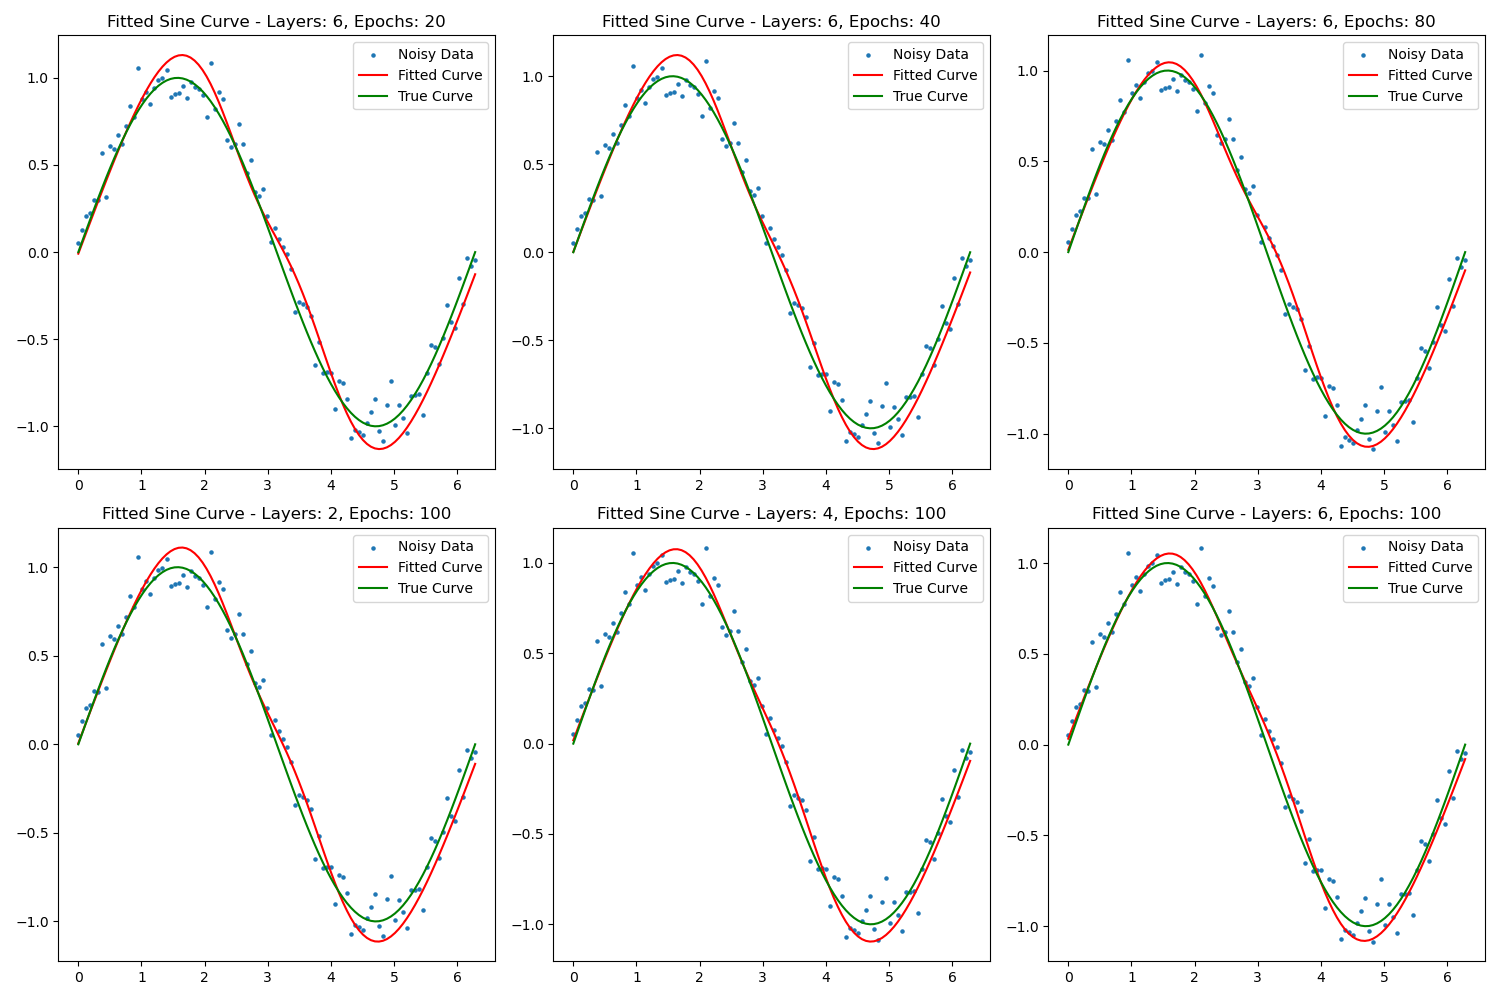
\includegraphics[width=\textwidth]{images/fits.png}
    \caption{Fitting a Noisy Sinusoid (Noise level = 0.1)}
    \label{t1}
\end{figure}

\begin{figure}[hbt!]
    \centering
    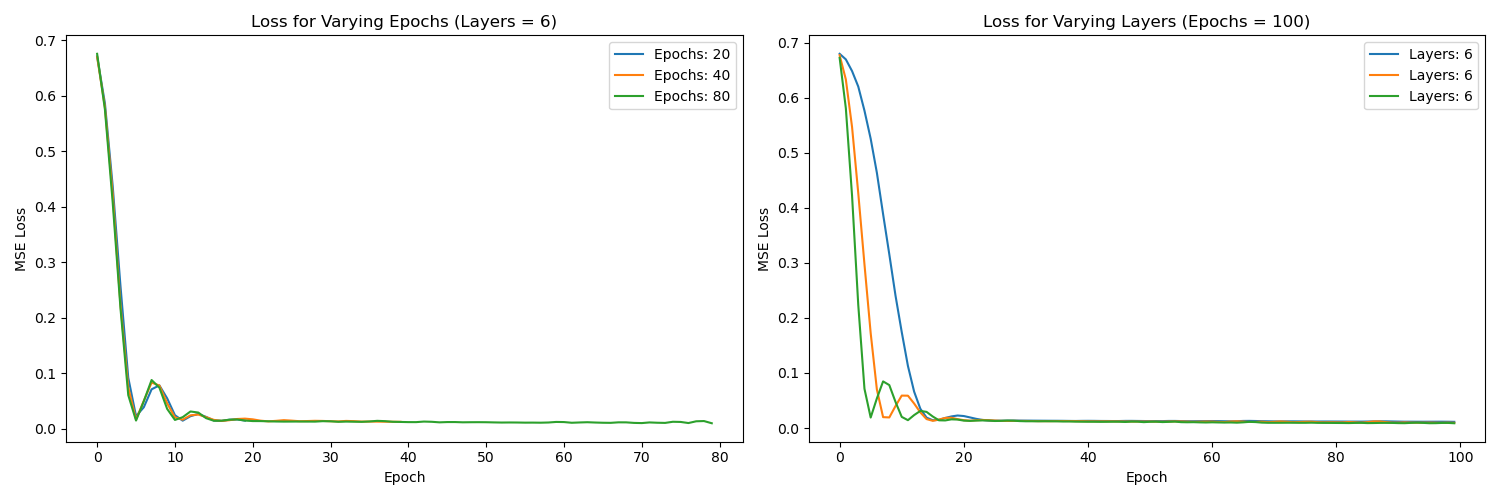
\includegraphics[width=\textwidth]{images/mses.png}
    \caption{MSE Loss}
    \label{t2}
\end{figure}

\FloatBarrier

\subsection{Analogous Classical NN}

Kerr-like transformation achieved by conditional rotation with angular velocity proportional to radius (value of the coordinate for 1D). The trainable parameter $\kappa$ is the proportionality constant.

\begin{figure}[hbt!]
    \centering
    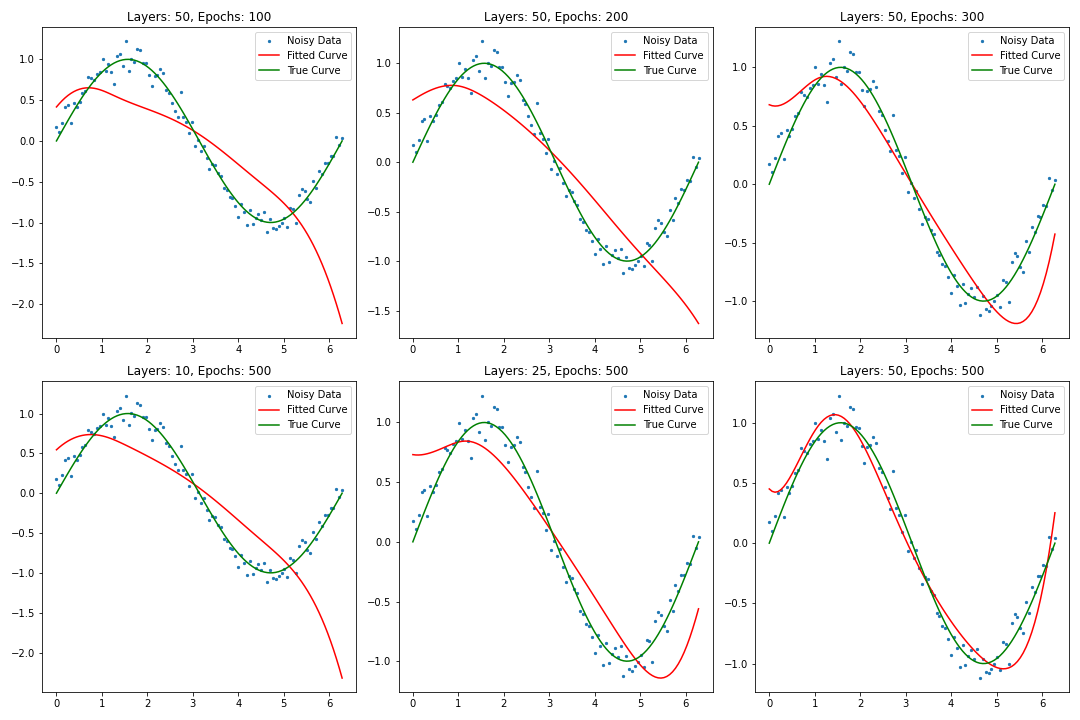
\includegraphics[width=\textwidth]{images/fits_classical.png}
    \caption{Fitting a Noisy Sinusoid (Noise level = 0.1)}
    \label{t3}
\end{figure}

\begin{figure}[hbt!]
    \centering
    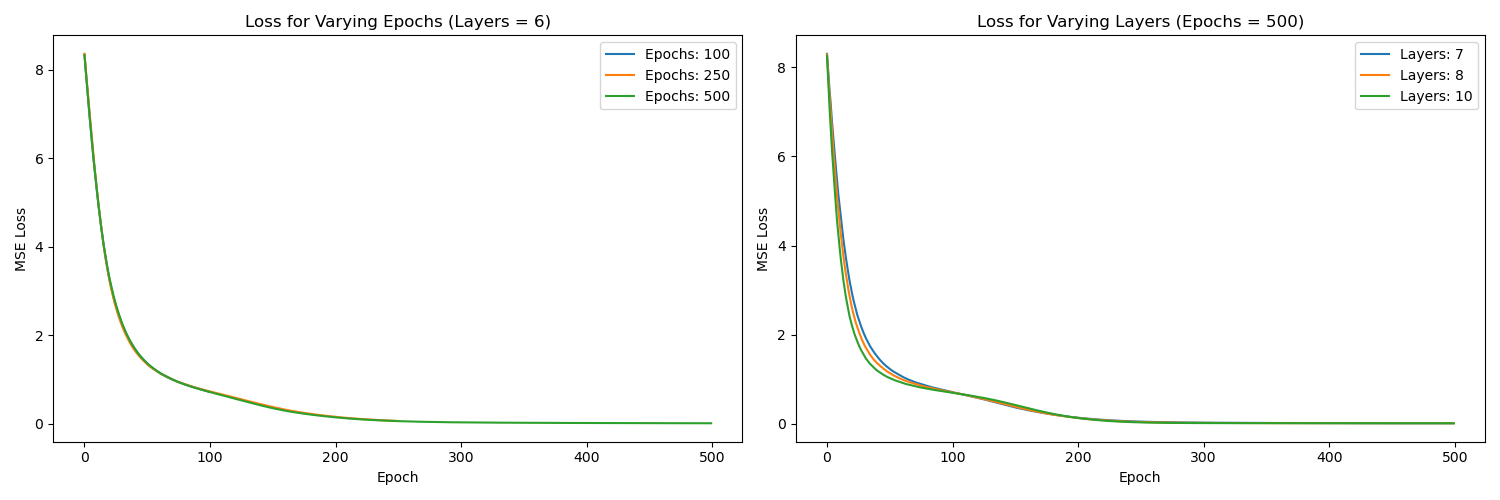
\includegraphics[width=\textwidth]{images/mses_classical.png}
    \caption{MSE Loss}
    \label{t4}
\end{figure}

\FloatBarrier

\subsection{Training and Validation MSE Comparision}
Choosing the two models from both scenarios to compare.

\begin{figure}[hbt!]
    \centering
    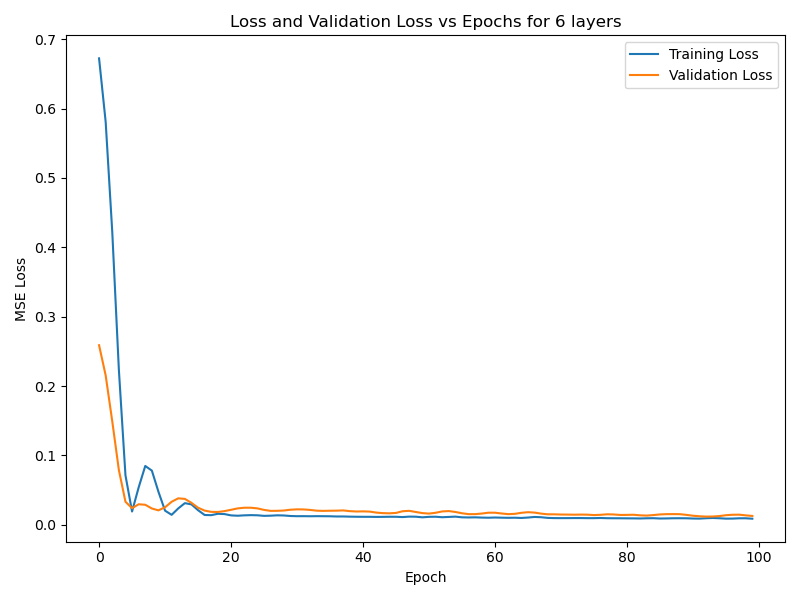
\includegraphics[width=0.75\textwidth]{images/mse_with_val.png}
    \caption{MSE Loss with 6 Layers and 100 epochs (QNN)}
    \label{t5}
\end{figure}

\begin{figure}[hbt!]
    \centering
    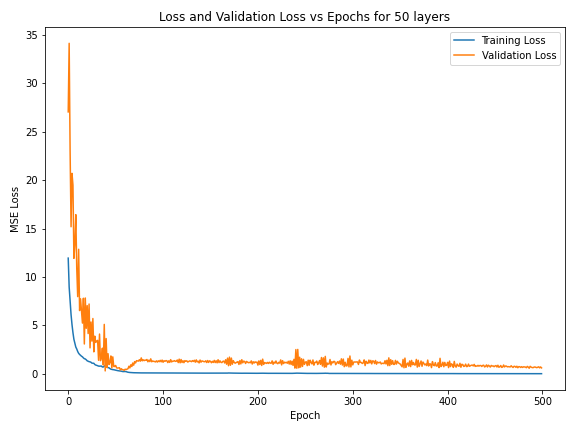
\includegraphics[width=0.75\textwidth]{images/mse_with_val_classical.png}
    \caption{MSE Loss with 8 Layers and 500 epochs (classical NN)}
    \label{t6}
\end{figure}

\FloatBarrier

\bibliographystyle{plain}
\bibliography{ref}

\end{document}


